\nomenclature[A]{LDC}{Low Duty Cycle}
\nomenclature[A]{DAA}{Detect and Avoid}
\nomenclature[A]{EIRP}{Equivalent Isotropically Radiated Power}

In this chapter, we discuss the duty cycle requirements for UWB and determine if platooning application requirements meet the duty cycle requirements for UWB.

To permit the use of Ultra Wide Band (UWB) but mitigate the possibility/effect of interference with other systems, two main approaches have been adopted which include Low Duty Cycle (LDC), and Detect and Avoid (DAA). LDC in which UWB equipment must limit the relative time for which it is transmitting. Detect and Avoid (DAA) in which UWB systems listen for other UWB transmissions before they transmit. The LDC requirement needs to be met when using Band 3 of UWB wherein the center frequency is 4488 MHz. LDC and DAA requirements have to be met when using Band 1, Band 2 and Band 11 of UWB wherein the center frequencies are 3432 MHz, 3960 MHz, and 8712 MHz respectively as shown in Figure \ref{fig:UWBRegulations}. It is to be noted that Detect and Avoid is not supported by DecaWave DW1000, the hardware used for the implementation of the thesis. The channels supported by DecaWave DW1000 are as shown in the Figure \ref{fig:ChannelsDecawaveDW1000}.
From the Figure \ref{fig:UWBRegulations} and Figure \ref{fig:ChannelsDecawaveDW1000}, we can infer that LDC regulations need to be met when using Channels 1, 2, 3 and 4 of DecaWave DW1000, and the same is not required when operating in Channels 5 and 7.
\begin{figure}[htbp]
    \begin{center}
        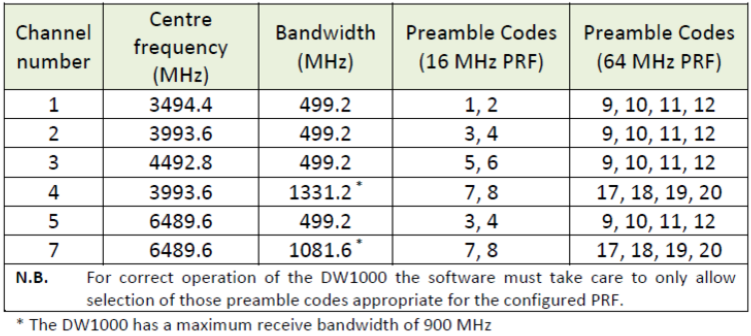
\includegraphics[width=1\textwidth]{figures/Picture2.png}
        \caption[Channels supported by DecaWave DW1000]{Channels supported by DecaWave DW1000 \protect\cite{DW1000UserManual}}
        \label{fig:ChannelsDecawaveDW1000}
    \end{center}
\end{figure}

\begin{figure}[htbp]
    \begin{center}
        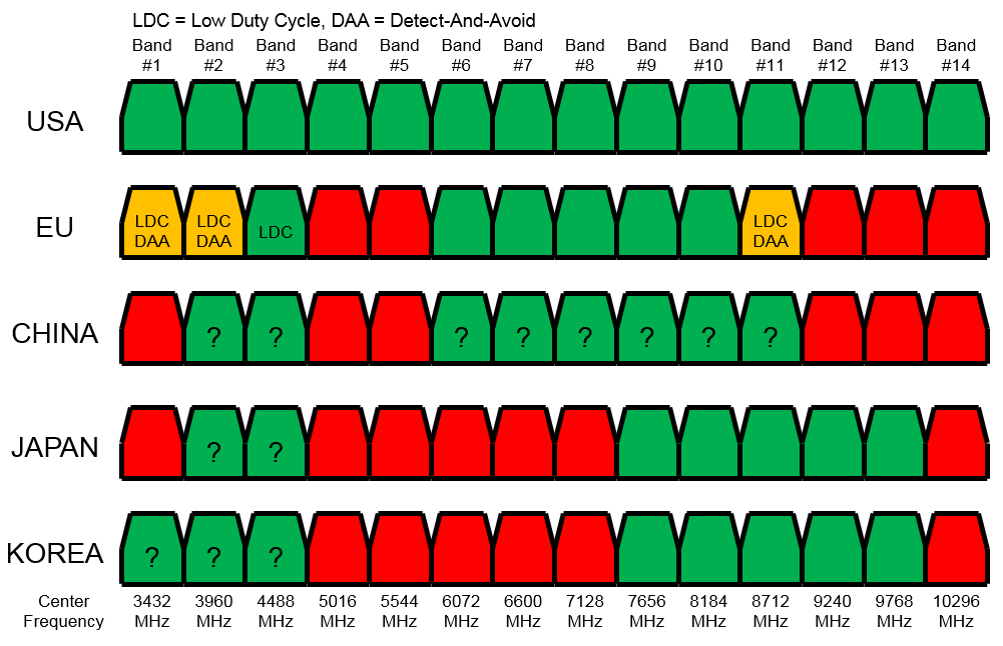
\includegraphics[width=1\textwidth, scale=0.7]{figures/Picture1.png}
        \caption{UWB Regulations, Source: F.Leong, NXP Semiconductors}
        \label{fig:UWBRegulations}
    \end{center}
\end{figure}

\section{Low Duty Cycle}
In Europe, the Electronic Communications Committee - one of CEPT's (European Conference of Postal and Telecommunications
Administrations) working committees dealing with radio spectrum use and telecommunications numbering\/ addressing, specifies technical requirements for LDC mitigation technique, enabling operation at -41.3 dBm /MHz Equivalent Isotropically Radiated Power (EIRP) within the band 3.4 - 4.8 GHz \cite{ECCDecision}. A device implementing LDC is a UWB device that meets the requirements as shown in Table ~\ref{fig:ECCDefLDC}.

\begin{table}[htbp]
    \begin{center}
        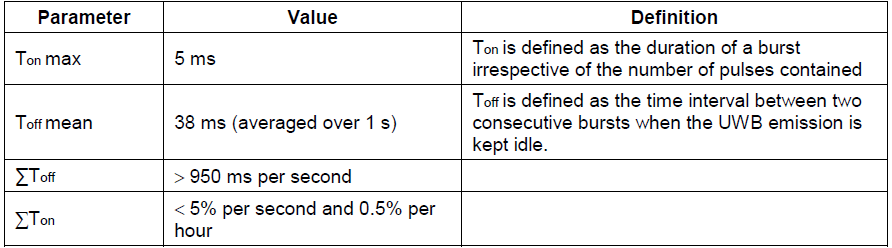
\includegraphics[width=1\textwidth]{figures/Picture3.png}
        \caption[ECC Definition of Low Duty Cycle Operation]{ECC Definition of Low Duty Cycle Operation \protect\cite{ECCDecision}}
        \label{fig:ECCDefLDC}
    \end{center}
\end{table}

To determine if LDC requirement can be met by truck platooning application, let's consider the UWB PHY frame structure and the application requirements.

\section{UWB PHY and Platooning Application}
UWB PHY frame structure is as shown in Figure \ref{fig:UWBPHYframeStructure}. According to the IEEE 802.15.4a UWB standard, the mandatory SHR Preamble base rate is 1.01 Msymbols/s and 0.25 Msymbol/s. The PHR is sent at 850 kb/s for all data rates greater than or equal to 850 kb/s and at 110 kb/s for the data rate of 110 kb/s.
The data field is transferred in MAC format as shown in Figure ~\ref{fig:MACMessageFormat} at the data rate defined experimentally. 

In truck platooning application, if we consider leading truck and the following truck, VFM (leading truck to the following truck) and PSM (following truck to the leading truck) are exchanged every 40 ms with a particular offset as shown in Figure \ref{fig:MessageExchangePlatooningApplication}.

Figure \ref{fig:DW1000SymbolDuration} shows the symbol durations for various configurations of PRF and data rate, which are used to calculate the LDC requirement for the truck platooning application.

\begin{figure}[htbp]
    \begin{center}
        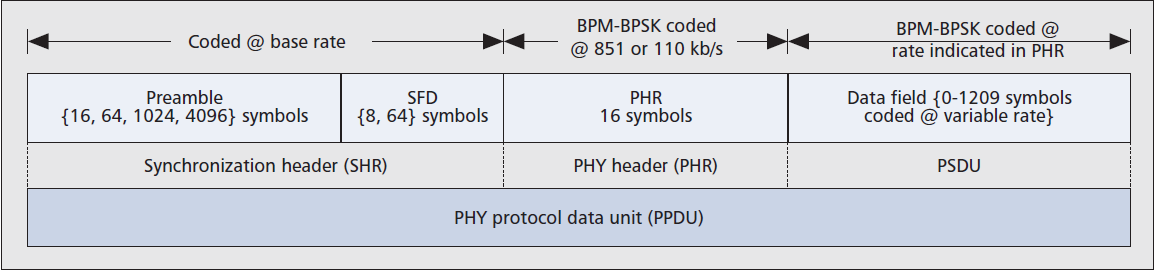
\includegraphics[width=1\textwidth]{figures/Picture4.png}
        \caption[UWB PHY Frame Structure]{UWB PHY Frame Structure \protect \cite{karapistoli2010overview}}
        \label{fig:UWBPHYframeStructure}
    \end{center}
\end{figure}

\begin{figure}[htbp]
    \begin{center}
        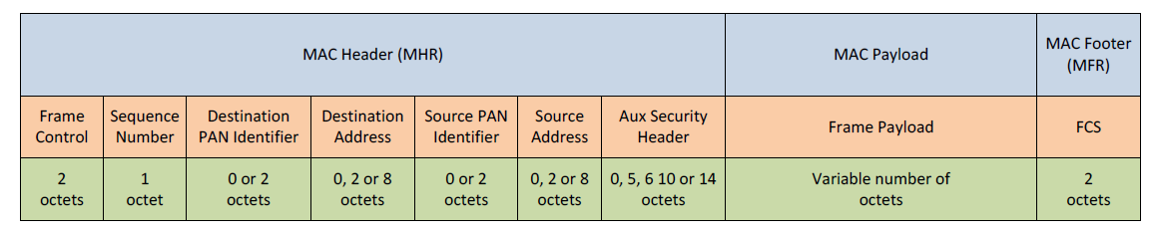
\includegraphics[width=1\textwidth]{figures/Picture5.png}
        \caption[802.15.4 - MAC Message Format]{802.15.4 - MAC Message Format \protect \cite{DW1000UserManual}}
        \label{fig:MACMessageFormat}
    \end{center}
\end{figure}

\begin{figure}[htbp]
    \begin{center}
        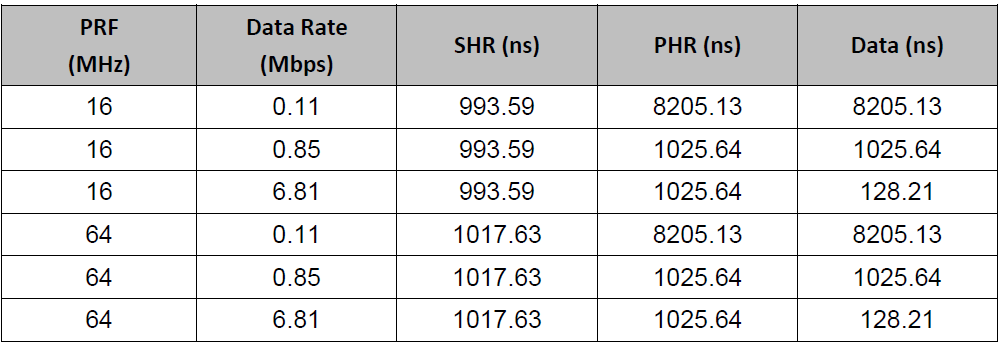
\includegraphics[width=1\textwidth]{figures/Picture7.png}
        \caption[DW1000 Symbol Durations]{DW1000 Symbol Durations \protect \cite{DW1000DataSheet}}
        \label{fig:DW1000SymbolDuration}
    \end{center}
\end{figure}

\section{LDC Calculation for the Truck Platooning Application}

According to the LDC requirement as specified in Table \ref{fig:ECCDefLDC}, the transmitter can be on for 50 ms of a second and 18000 ms of an hour. To check if the truck platooning application meets the LDC requirement, let's consider the typical platooning payloads of 60 bytes (1 packet/message) and 160 bytes (2 packets/message). Here, 60 bytes and 160 bytes corresponds to the minimum and maximum platooning payload of the current Eco-Twin Truck platooning implementation \cite{euTPC}.

For the calculation of the Ton times for 6.8 Mbps, following values are used for various parameters.
\vspace{0.2cm}
\\Preamble Length = 64 Symbols \\
Data Rate = 6.8 Mbps \\
Bit Rate = 6800 \\
PHR Rate = 850 \\
PHR = 19 bits \\
SFD length = 8 Symbols \\
PRF = 16 MHz (Symbol Duration = 993.59 ns) or 64 MHz(Symbol Duration = 1017.63 ns)\\

Let us calculate the respective Ton times for the following scenarios using Equation~\ref{eq:PreambleDuration} and Equation~\ref{eq:maxFrameDuration}. 
\begin{equation}
Preamble Duration = (preambleLength + sfdLength)* preambleSymbolDuration
\label{eq:PreambleDuration}
\end{equation}
\begin{equation}
maxFrameDuration = preambleDuration + 19/phrRate + packetSize * 8/ bitRate
\label{eq:maxFrameDuration}
\end{equation}

\begin{itemize}
    \item \textbf{Scenario 1: 60 bytes payload, 64 MHz PRF} For Scenario 1, we can determine that the maximum frame duration is 0.1662 ms. Considering a single mirror, 25  messages are transmitted in a second because of the platooning application requirement of 25 Hz. For 1 second, the total Ton time is 4.1550 ms out of the available 50 ms and for 1 hour, the total Ton time is 14958 ms out of the available 18000 ms. Since the max duration of a burst is always less than 5 ms. LDC requirement is met in this scenario. 
    
    \item \textbf{Scenario 2: 60 bytes payload, 16 MHz PRF} For Scenario 2, we can determine that the maximum frame duration is 0.1645 ms. For 1 second, the total Ton time is 4.1125 ms out of the available 50 ms and for 1 hour, the total Ton time is 14805 ms out of the available 18000 ms. Since the max duration of a burst is always less than 5 ms. LDC requirement is met in this scenario too. 
    
    \item \textbf{Scenario 3: 160 bytes payload, 64 MHz PRF} For Scenario 3, we can determine that the maximum frame duration is 0.3794 ms if we transmit two packets each of 80 bytes. For 1 second, the total Ton time is 9.4850 ms out of the available 50 ms and for 1 hour, the total Ton time is 34146 ms out of the available 18000 ms. LDC requirement is not met in this scenario because of the hourly constraint. 
    
    \item \textbf{Scenario 4: 160 bytes payload, 16 MHz PRF} For Scenario 4, we can determine that the maximum frame duration is 0.3760 ms if we transmit two packets each of 80 bytes. For 1 second, the total Ton time is 9.4000 ms out of the available 50 ms and for 1 hour, the total Ton time is 33840 ms out of the available 18000 ms. LDC requirement is not met in this scenario because of the hourly constraint. 
    
\end{itemize}

Hence the UWB system for truck platooning will meet the LDC requirement according to the regulations when 6.8 Mbps data rate, 60 bytes minimum platooning payload, minimum preamble length, and a UWB transceiver mounted on a single mirror is considered. 

\vspace{3cm}
Similarly, we can calculate Ton times for 850 Kbps and 110 Kbps using Equation~\ref{eq:PreambleDuration} and Equation~\ref{eq:maxFrameDuration}. For the calculation of Ton times for 850 Kbps, following values are used for various parameters.
\vspace{0.2cm}
\\Preamble Length = 256 Symbols \\
Data Rate = 850 Kbps \\
Bit Rate = 850 \\
PHR Rate = 850 \\
PHR = 19 bits \\
SFD length = 8 Symbols \\
PRF = 16 MHz (Symbol Duration = 993.59 ns) or 64 MHz(Symbol Duration = 1017.63 ns)\\

For the calculation of Ton times for 110 Kbps, following values are used for various parameters.
\vspace{0.1cm}
\\Preamble Length = 2046 Symbols \\
Data Rate = 110 Kbps \\
Bit Rate = 110 \\
PHR Rate = 110 \\
PHR = 19 bits \\
SFD length = 8 Symbols \\
PRF = 16 MHz (Symbol Duration = 993.59 ns) or 64 MHz(Symbol Duration = 1017.63 ns)\\


% Please add the following required packages to your document preamble:
% \usepackage{multirow}
% \usepackage{graphicx}
\begin{table}[]
    \centering
    \caption{Ton with respect to data rates for Platooning application}
    \label{tab:Ton with respect to data rates for Platooning application}
    \resizebox{\textwidth}{!}{%
        \begin{tabular}{|l|c|c|c|c|}
            \hline
            \multirow{2}{*}{\textbf{Data Rate}} & \multicolumn{4}{c|}{\textbf{Ton Duration in milliseconds (calculated per hour)}}                                                                                                                                    \\ \cline{2-5} 
            & \multicolumn{1}{l|}{\textbf{60 bytes, 64 MHz PRF}} & \multicolumn{1}{l|}{\textbf{60 bytes, 16 MHz PRF}} & \multicolumn{1}{l|}{\textbf{160 bytes, 64 MHz PRF}} & \multicolumn{1}{l|}{\textbf{160 bytes, 16 MHz PRF}} \\ \hline
            \textbf{6.8 Mbps}                   & 14958                                              & 14805                                              & 34146                                               & 33840                                               \\ \hline
            \textbf{850 Kbps}                   & 77013                                              & 76446                                              & 187902                                              & 186768                                              \\ \hline
            \textbf{110 Kbps}                   & 601704                                             & 597132                                             & 1465218                                             & 1456092                                             \\ \hline
        \end{tabular}%
    }
\end{table}

Table \ref{tab:Ton with respect to data rates for Platooning application} summarizes the Ton durations with respect to data rates 6.8 Mbps, 850 Kbps and 110 Kbps for Platooning application. It is to be noted that the LDC requirement is not fulfilled for all scenarios when 850 Kbps or 110 Kbps is used because, for 1 hour, the total Ton time must be within 18000 ms. Only in the case of 6.8 Mbps, LDC requirement is met when 60 bytes minimum platooning payload, minimum preamble length and a UWB transceiver mounted on a single mirror is considered. 